\chapter{图表分析}\label{chap:figtbl}
文章中图表的类型比较丰富,可以粗略分为视觉型插图和文字型插图,以下从宏观和微观两个角度来分析该文章的图表。

\section{从宏观角度分析}
从宏观的角度来看,我们可以从以下4个方面进行分析:
\begin{enumerate}
\item
插图的数量,文章共有9页,共有9张插图,平均每页一张插图,让读者阅读起来不会产生视觉疲劳
\item
插图的类型,文中视觉型插图(如图~\ref{fig:visualp})有4张,文字型插图(公式和表格,如图~\ref{fig:textp})共5张,类型配比接近1:1,类型均衡
\begin{figure}[!htbp]
    \centering
    \begin{subfigure}[b]{0.35\textwidth}
      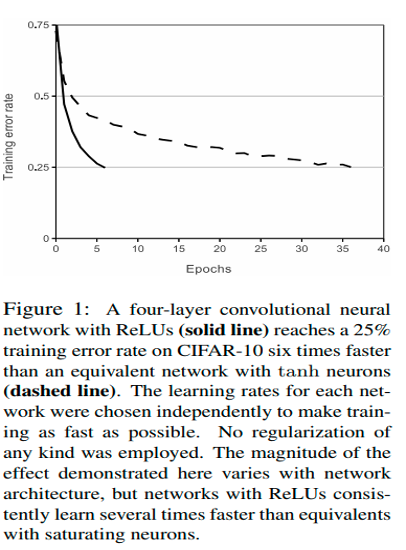
\includegraphics[width=\textwidth]{visualp1}
      \caption{}
      \label{fig:oaspl_a}
    \end{subfigure}%
    ~% add desired spacing
    \begin{subfigure}[b]{0.35\textwidth}
      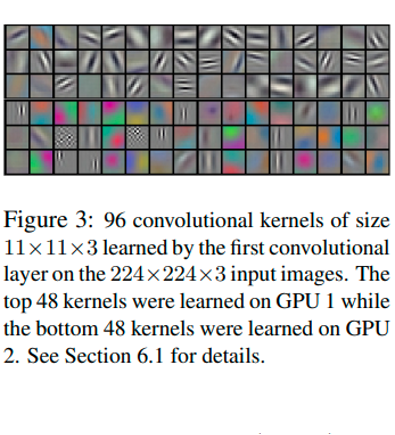
\includegraphics[width=\textwidth]{visualp2}
      \caption{}
      \label{fig:oaspl_b}
    \end{subfigure}
    \\% line break
    \begin{subfigure}[b]{0.35\textwidth}
      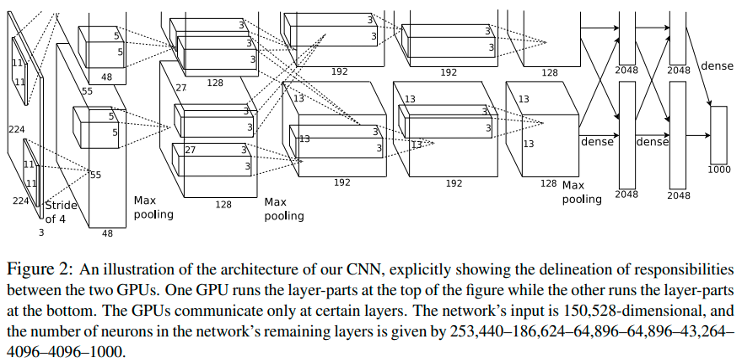
\includegraphics[width=\textwidth]{visualp3}
      \caption{}
      \label{fig:oaspl_c}
    \end{subfigure}%
    ~% add desired spacing
    \begin{subfigure}[b]{0.35\textwidth}
      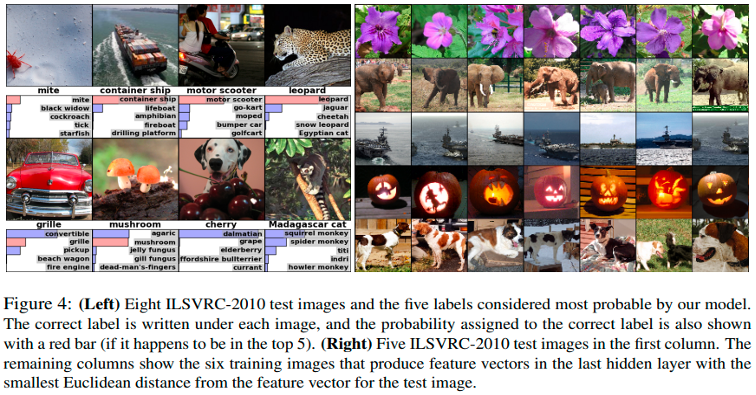
\includegraphics[width=\textwidth]{visualp4}
      \caption{}
      \label{fig:oaspl_d}
    \end{subfigure}
    \caption{视觉型插图}
    \label{fig:visualp}
\end{figure}

\begin{figure}[!htbp]
    \centering
    \begin{subfigure}[b]{0.35\textwidth}
      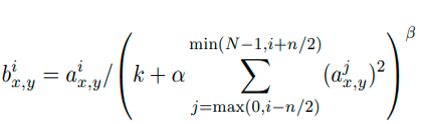
\includegraphics[width=\textwidth]{textp1}
      \caption{}
      \label{fig:oaspl_a}
    \end{subfigure}%
    ~% add desired spacing
    \begin{subfigure}[b]{0.35\textwidth}
      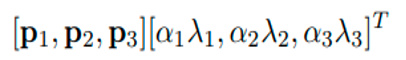
\includegraphics[width=\textwidth]{textp2}
      \caption{}
      \label{fig:oaspl_b}
    \end{subfigure}
    \\% line break
    \begin{subfigure}[b]{0.35\textwidth}
      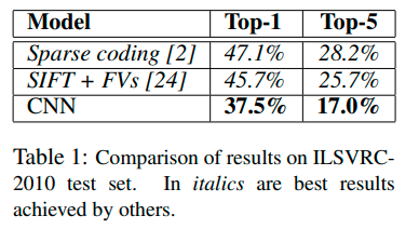
\includegraphics[width=\textwidth]{textp4}
      \caption{}
      \label{fig:oaspl_c}
    \end{subfigure}%
    ~% add desired spacing
    \begin{subfigure}[b]{0.35\textwidth}
      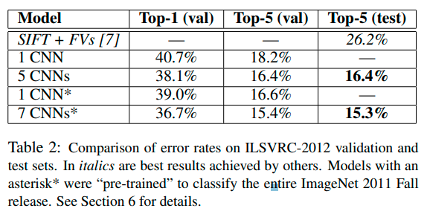
\includegraphics[width=\textwidth]{textp5}
      \caption{}
      \label{fig:oaspl_d}
    \end{subfigure}
    ~% add desired spacing
    \begin{subfigure}[b]{0.35\textwidth}
      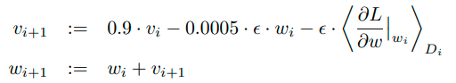
\includegraphics[width=\textwidth]{textp3}
      \caption{}
      \label{fig:oaspl_d}
    \end{subfigure}
    \caption{文本型插图。(a) 位于3.3节 ,(b) 位于4.1节,(c) 位于第6节,(d) 位于第6节,(e)位于第5节。}
    \label{fig:textp}
\end{figure}

\item
插图在文中的位置分布,文章分为7部分,其中第3-6节是主体部分,在3.1节、3.5节、第5节、6.1节中各有一张视觉型插图,在3.3节、4.1节、第5节各有一个公式,第6节有两张表格。不难发现:图表在各节的分布也很均衡,同一小节最多不会多于2张插图,且除第6节外,每一节插图的类型都不一样,同时也没有图表的堆叠,给读者带来了良好的视觉体验,且能实时结合图表,有助于对文章内容的理解把握。
\item
内容和插图的排版,文中的插图和文字内容部分大部分很合理,除了第6节中的两张表格,如图~\ref{fig:improper}所示。

其中表格的位置对文字表述部分造成了冲击,使得一个单词跨两行的现象增多,让排版变得有些混乱,一定程度上影响了读者的阅读体验。我们认为,让文字环绕在表格上下,同时将表格的标题行数减少(同时增加每行容纳的词数),带来的视觉效果更好。
\end{enumerate}
% 1.	插图的数量,文章共有9页,共有9张插图,平均每页一张插图,让读者阅读起来不会产生视觉疲劳
% 2.	插图的类型,文中视觉型插图有4张,文字型插图(公式和表格)共5张,类型配比接近1:1,类型均衡 
% 3.	插图在文中的位置分布,文章分为7部分,其中第3-6节是主体部分,在3.1节、3.5节、第5节、6.1节中各有一张视觉型插图,在3.3节、4.1节、第5节各有一个公式,第6节有两张表格。不难发现:图表在各节的分布也很均衡,同一小节最多不会多于2张插图,且除第6节外,每一节插图的类型都不一样,同时也没有图表的堆叠,给读者带来了良好的视觉体验,且能实时结合图表,有助于对文章内容的理解把握。 
% 4.	内容和插图的排版,文中的插图和文字内容部分大部分很合理,除了第6节中的两张表格,如图~\ref{fig:improper}所示:
\begin{figure}[!htbp]
	\centering
	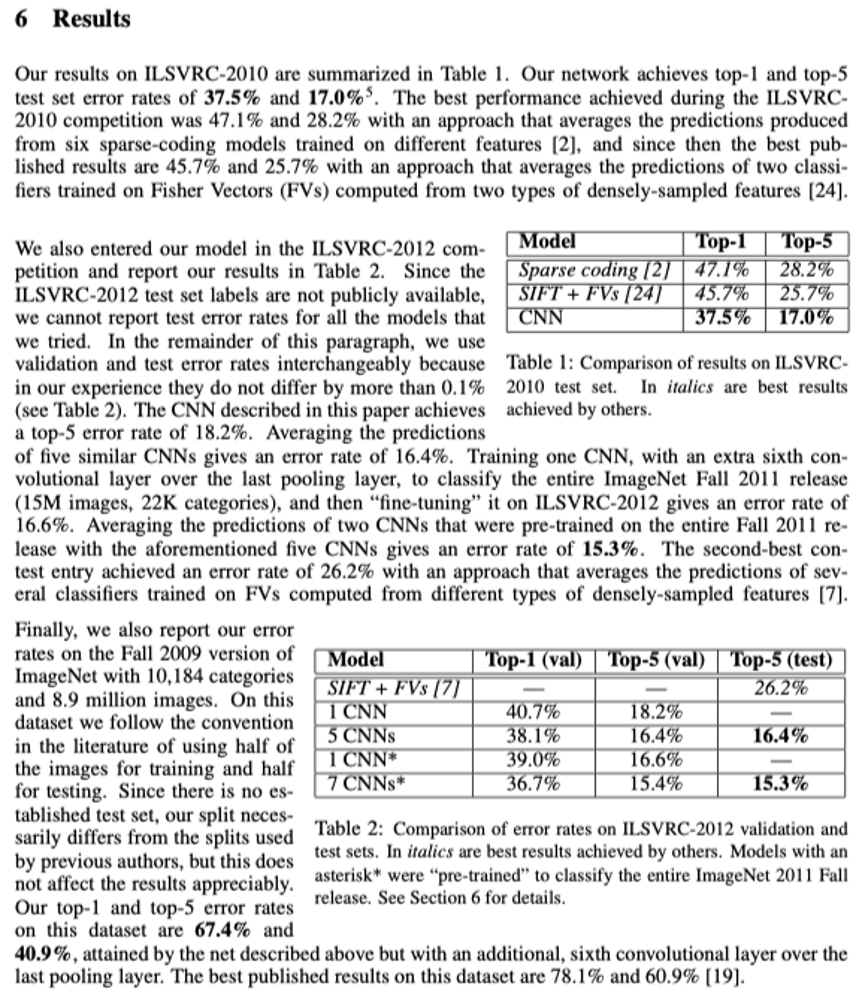
\includegraphics[width=\textwidth]{improper}
	\caption{不合理的表格排版}
	\label{fig:improper}
\end{figure}

\section{从微观角度分析}
从微观的角度来看,可以从以下2个方面进行分析。
\begin{enumerate}
\item 视觉型插图,视觉型插图包含了图表、图示、图片,每张插图的标题都清楚的对插图进行了说明,做到了自明,同时图标、图示结构简洁清晰,图片的组合清晰美观,不得不说,该文的视觉型插图做的很棒,让读者能够更加直观的理解文章提出的CNN网络以及它的功能;
\item 文本型插图,其中包含了公式和表格,公式并没有大量使用,只是在论述过程中恰如其分的用来准确的表达概念,且所使用的公式形式简单,对大多数读者而言,增强了可读性,更易于理解;表格做到了自明,所表达的内容也不冗余,通过与其他模型的量化对比,让读者清晰直观的掌握到CNN网络的性能,但表格还有改进的空间,例如改为如表~\ref{tab:tbl1}、表~\ref{tab:tbl2}形式:

\end{enumerate}
% Table generated by Excel2LaTeX from sheet 'Sheet1'
\begin{table}[!htbp]
  \renewcommand\arraystretch{0.8}
  \centering
  \caption{修改后的Table 1}
    \begin{tabular}{p{10.915em}rr}
    \toprule
    \textbf{Model} & \multicolumn{1}{c}{\textbf{Top-1}} & \multicolumn{1}{c}{\textbf{Top-5}} \\
    \midrule
    \textit{Sparse coding [2]} & \multicolumn{1}{c}{\textit{47.10\%}} & \multicolumn{1}{c}{\textit{28.20\%}} \\
    \textit{SIFT+FVs [24]} & \multicolumn{1}{c}{\textit{45.70\%}} & \multicolumn{1}{c}{\textit{25.70\%}} \\
    \textbf{CNN} & \multicolumn{1}{c}{\textbf{37.50\%}} & \multicolumn{1}{c}{\textbf{17.00\%}} \\
    \midrule
    \multicolumn{3}{p{22.415em}}{Table 1: Comparison of results on ILSVRC2010 test set. In italics are best results achieved by others} \\
    \end{tabular}%
  \label{tab:tbl1}%
\end{table}%

% Table generated by Excel2LaTeX from sheet 'Sheet1'
\begin{table}[!htbp]
  \renewcommand\arraystretch{0.8}
  \centering
  \caption{修改后的Table 2}
    \begin{tabular}{p{8.215em}lp{8.215em}rp{8.215em}cp{8.215em}c}
    \toprule
    \textbf{Model} & \multicolumn{1}{c}{\textbf{Top-1(val)}} & \multicolumn{1}{c}{\textbf{Top-5(val)}} & \multicolumn{1}{c}{\textbf{Top-5(test)}} \\
    \midrule
    \textit{SIFT+FVs[7]} & \multicolumn{1}{p{8.215em}<{\centering}}{—} & \multicolumn{1}{c}{—} & \multicolumn{1}{c}{\textit{28.20\%}} \\
    1CNN  & \multicolumn{1}{c}{40.70\%} & \multicolumn{1}{c}{18.20\%} & \multicolumn{1}{c}{—} \\
    5CNNs & \multicolumn{1}{c}{38.10\%} & \multicolumn{1}{c}{16.40\%} & \multicolumn{1}{c}{\textbf{16.40\%}} \\
    1CNN* & \multicolumn{1}{c}{39.00\%} & \multicolumn{1}{c}{16.60\%} & \multicolumn{1}{c}{—} \\
    7CNNs* & \multicolumn{1}{c}{36.70\%} & \multicolumn{1}{c}{15.40\%} & \multicolumn{1}{c}{\textbf{15.30\%}} \\
    \midrule
    \multicolumn{4}{p{32.92em}}{Table 2: Comparison of error on ILSVRC-2012 validation and test sets. In italics are best results achieved by others. Models with an asterisk* were “pre-trained” to classify the entire ImageNet 2011 Fall release. See Section 6 for details.  } \\
    \end{tabular}%
  \label{tab:tbl2}%
\end{table}%

